\documentclass[12pt]{report}

\usepackage{commands}


\begin{document}

\large

\begin{center}
 Math 569 Homework 6\\
 Due May 31\\
 By Marvyn Bailly\\
\end{center}

\normalsize

\hrule

%---------------%
%---Problem 1---%
%---------------%

%--status--$

\def\p{\varPsi}
\def\n{\nabla}

\begin{problem}
    Consider the sound waves governed by
    \[
        \ppn{2}{}{t} \p = c^2 \n^2 \p, ~~ \n^2= \frac{1}{r}\pp{}{r}\paren{r\pp{}{r}} + \frac{1}{r^2}\ppn{2}{}{\theta} + \ppn{2}{}{z},
    \] 
    in a circular cylinder of radius $a$ and length $L$ with
    \[
        \p = 0 ~\text{at}~r=a;~\p=0 ~\text{at}~z=0,L.
    \]
    Assume that the sound produced in this tube is symmetric, i.e. no $\theta$ dependence. Find the lowest three frequencies. Take $c=300$m/s, $a=1$cm, and $L=0.5$m.
\end{problem}

\begin{solution}
    
    \noindent
    Consider the sound waves governed by
    \[
        \ppn{2}{}{t} \p = c^2 \n^2 \p, ~~ \n^2= \frac{1}{r}\pp{}{r}\paren{r\pp{}{r}} + \frac{1}{r^2}\ppn{2}{}{\theta} + \ppn{2}{}{z},
    \] 
    in a circular cylinder of radius $a$ and length $L$ with
    \[
        \p = 0 ~\text{at}~r=a;~\p=0 ~\text{at}~z=0,L.
    \]
    We will assume that the sound produced in this tube is symmetric, i.e. there is no $\theta$ dependence. Let's use the separation of variables method to solve this PDE so we assume that 
    \[
        \p(r,\theta,z,t) = T(t)\psi (r,z).        
    \]
    Plugging this into our PDE and rearranging terms yields
    \[
        \frac{T''}{c^2T} = \frac{\nabla^2 \psi}{\psi} = -\lambda^2,
    \]
    where $\lambda$ is a positive constant. This breaks down into two problems
    \[
        \frac{T''}{c^2T} = -\lambda^2,
    \]
    and
    \[
        \frac{\nabla^2 \psi}{\psi} = -\lambda^2.
    \]
    To solve the first equation, we rearrange the terms to get
    \[
        T'' + c^2\lambda^2 T = 0.
    \]
    Solve for $T$ gives
    \[
        T(t) = A\sin(c\lambda t) + B\cos(c\lambda t) = A\sin(\omega t) + B\cos(\omega t).
    \]
    Now we return to the spatial problem. Note that we removed the $\theta$ dependence by our assumption and thus we take
    \[
        \psi(r,z) = R(r)Z(z),
    \]
    allowing us to use the separation of variables. This gives
    \[
        \frac{\nabla^2 \psi}{\psi} = \frac{1}{rR}\pp{}{r}\paren{rR'} + \frac{Z''}{Z} = - \lambda^2,
    \]
    which is only true if
    \[
        \frac{Z''}{Z} = - \lambda^2 - \frac{1}{rR}\pp{}{r}(rR') = -\xi^2,
    \]
    where $\xi$ is a positive constant. Now we can solve for $Z$ using the same method present to solve $T$ to get
    \[
        Z(z) = C\sin(\xi z) + D\cos(\xi z).
    \]
    Now we can apply the boundary condition that $\p = 0 $ at $z=0$ which gives that $D=0$. Next, we apply the boundary condition that $\p =0$ at $z=L$ which gives
    \[
        Z(L) = C\sin(\xi L) = 0,
    \] 
    and thus
    \[
        \xi = \frac{n \pi}{L},
    \]
    for $n=1,2,\dots$. Thus we have found that
    \[
        Z_n = \sin\paren{\frac{n\pi}{L}z},
    \]
    where we let $C=1$. Now returning to the $R$ equation we have
    \[
        \frac{1}{rR}\pp{}{r}(rR') = \xi^2 - \lambda^2 = -\alpha^2.
    \]
    Then rearranging the terms we get
    \[
        R'' + \frac{1}{r}R' + \alpha^2 R = 0.
    \]
    Now applying the change of variables $s=\alpha r$, we get
    \[
        s^2 R''(s) + sR'(s) + s^2R(s) = 0.
    \]
    Noticing that this is a Bessel differential equation we get the solutions
    \[
        R(r) = c_1 J_0(\alpha r) + c_2 Y_0(\alpha r),
    \]    
    where $J_0$ and $Y_0$ are Bessel functions of the first and second kind respectively. Now applying the boundary condition $\p = 0$ at $r=a$, we see that $c_2=0$ since $Y_0 \to -\infty$ as $t\to 0$. Then taking $c_1 = 1$ we get
    \[
        R(r) = J_0(\alpha r).
    \]
    Note that we require $R(a) = 0$ and thus we need the zeros of the Bessel function of the first kind $J_0$. We will later compute these numerically but for now, we consider the solution to be 
    \[
        R_m(r) = J_0(\alpha r).
    \]
    Thus we have the solution
    \[
        \p_{n,m}(r,\theta,z,t) = \paren{A\sin(\omega t) + B\cos(\omega t)}\sin\paren{\frac{n \pi}{L}z}R_m(r),
    \]
    or
    \[
        \p = \sum_{n,m=1}^{\infty}\paren{A\sin(\omega t) + B\cos(\omega t)}\sin\paren{\frac{n \pi}{L}z}R_m(r).
    \]
    Now recalling that
    \[
        -\lambda^2 + \xi^2 = -\alpha^2 \implies \lambda^2 = \xi^2 + \alpha^2,
    \]  
    and thus
    \[
        \omega_{n,m} = c\lambda_{n,m} = c\sqrt{\xi^2_n + \alpha^2_n}.
    \]
    The zeros of $J_0(x)$ are well known and using a good book about Bessel functions we find the first few zeros to be
    \[
        \begin{cases}
            s = 2.40482558, &m=1,\\
            s = 5.52007811, &m=2,\\
            s = 8.653727913, &m=3.
        \end{cases}
    \] 
    Since $a = 0.01$ we have
    \[
        \begin{cases}
            \alpha_1 = 240.482556,\\
            \alpha_2 = 552.007811,\\
            \alpha_3 = 865.372791.\\
        \end{cases}
    \]
    We are searching for the three lowest frequencies and noticing that $\xi_1 = 2\pi, \xi_2 = 4\pi,\and \xi_3=6\pi,$ and thus the three lowest frequencies are given by $\alpha_1$ and $\xi_{1,2,3}$. Therefore we have found the three lowest frequencies to be
    \[
        \begin{cases}
            \omega_{1,1} = 300 \sqrt{(2\pi)^2 + \paren{240.482556}^2} \approx 72169 \mathrm{Hz},\\
            \omega_{2,1} = 300 \sqrt{(4\pi)^2 + \paren{240.482556}^2} \approx 72243 \mathrm{Hz},\\
            \omega_{3,1} = 300 \sqrt{(6\pi)^2 + \paren{240.482556}^2} \approx 72366 \mathrm{Hz},
        \end{cases}
    \]





\end{solution}

%----------------------------------------------------------------------------------------------------%
%\vskip 20pt
\newpage

%---------------%
%---Problem 2---%
%---------------%

%--status--$

\begin{problem}
    Consider the wave function $\p$ for an electron of mass $\mu$ in a sphere surrounded by an infinite potential at a radius a from the nucleus, which just means that $\p = 0$ at $r=a$.
    \[
        i\hbar \pp{}{t}\p = - \frac{\hbar^2}{2\mu}\nabla^2\p.
    \] 
    Find the energy levels for the symmetric case, where $\p$ does not depend on $\theta$ and $\phi$. Your answer should be exact and in terms of the parameters given.
\end{problem}

\begin{solution}

    \noindent
    Consider the wave function $\p$ for an electron of mass $\mu$ in a sphere surrounded by an infinite potential at a radius a from the nucleus, which just means that $\p = 0$ at $r=a$.
    \[
        i\hbar \pp{}{t}\p = - \frac{\hbar^2}{2\mu}\d^2\p.
    \]
    We wish to find the energy levels for the symmetric case and thus $\p$ does not depend on $\theta$ and $\phi$. We will use the separation of variables method to solve this PDE so we assume that
    \[
        \p = T(t)\psi.
    \]
    Plugging this back into the PDE and rearranging terms yields
    \[
        -\frac{2 i \mu}{\hbar} \frac{T'}{T} = \frac{\nabla^2 \psi}{\psi} = -\lambda^2, 
    \]
    where $\lambda$ is a positive constant. This gives the ODE
    \[
        T' + \frac{i \hbar \lambda^2}{2\mu}T = 0,
    \]
    which has the solution
    \[
        T = Ae^{\frac{-i \hbar \lambda^2}{2\mu}t}.
    \]
    Now returning to 
    \[
        \frac{\nabla^2 \psi}{\psi} = -\lambda^2,
    \]
    where we note that $\psi$ only depends on $r$ since we are in the symmetric case. Thus we have
    \[
        \frac{1}{r^2}\pp{}{r}\paren(r^2 R') = -\lambda^2 R.
    \]
    If we preform the change of variable $s=\lambda r$ we get 
    \[
        s^2R'' + 2sR' + s^2 R = 0.
    \]
    Noticing that this is the spherical Bessel function, we find the solution to be
    \[
        R(s) = Bj_0(s) + Cy_0(s),
    \]
    where $j_0$ and $y_0$ are the spherical Bessel functions of the first and second kind respectively. Since the boundary condition requires $\p = 0$ at $r=a$ we require $C=0$ and thus taking $B=1$ we have
    \[
        R(r) = j_0(\lambda r).
    \]
    Now recalling that
    \[
        j_0 = \frac{\sin(x)}{x},
    \]
    we have
    \[
        R(r) = \frac{\sin(\lambda r)}{\lambda r}.
    \]
    Now enforcing the boundary condition $\p =0$ at $r=a$ we get
    \[
        \frac{\sin(\lambda a)}{\lambda a} = 0 \implies \sin(\lambda a) = 0 \implies \lambda_n = \frac{n\pi}{a},
    \]
    under the assumption that $\lambda \neq 0$ and for $n=1,2,\dots$. From the class notes, we know that the quantized energy of a particle is given by
    \[
        E_n = \frac{\hbar^2}{2\mu}\lambda_n^2.
    \]
    Therefore the energy levels in the symmetric case are
    \[
        E_n = \frac{\hbar^2 n^2 \pi^2}{2\mu a^2}, \quad n=1,2,\dots.        
    \]
    Note that the solution to the original PDE is 
    \[
        \p = \sum_{n=1}^{\infty}e^{-\frac{iE_n}{\hbar}t}j_0\paren{\frac{n\pi}{a}r}.
    \]




\end{solution}

%----------------------------------------------------------------------------------------------------%
%\vskip 20pt
\newpage

%---------------%
%---Problem 3---%
%---------------%

%--status--$

\begin{problem}
    Consider the Legendre's equation:
    \[
        \dd{}{x} \paren{(1-x^2)\dd{}{x}y(x)} + n(n+1)y(x) = 0, ~ -1 \leq x \leq 1,
    \] 
    with the initial condition that $y(\pm1)$ are bounded. The solutions are the Legendre polynomials, $P_n(x)$, which are given by the Rodrigue's formula:
    \[
        P_n(x) = \frac{1}{2^n n!}\ddn{n}{}{x}(x^2 - 1)^n. 
    \]
    Compute the first four coefficients in the Legendre expansion (similar to Fourier sine or cosine series expansion):
    \[
        f(x) = \sum_{n=0}^{\infty} a_n P_n(x), ~\text{where}~ a_n = \frac{2n+1}{2}\int_{-1}^{1}f(x) P_n(x) \d x,
    \]
    for 
    \[
        f(x) = \begin{cases}
            0 \for -1<x<0,\\
            x ~\text{for}~ 0<x<1.
        \end{cases}
    \]
    Plot the approximation of the sum consisting of one, two, three and four terms along with the original function $f(x)$. 




\end{problem}

\begin{solution}

    \noindent
    We wish to compute the first four coefficients in the Legendre expansion of the form
    \[
        f(x) = \sum_{n=0}^{\infty} a_n P_n(x),
    \]
    where
    \[
        a_n = \frac{2n+1}{2}\int_{-1}^{1}f(x) P_n(x) \d x,
    \]
    and
    \[
        P_n(x) = \frac{1}{2^n n!}\ddn{n}{}{x}(x^2 - 1)^n,    
    \]
    for 
    \[
        f(x) = \begin{cases}
            0 \for -1<x<0,\\
            x ~\text{for}~ 0<x<1.
        \end{cases}
    \]
    The first coefficient in the expansion is
    \begin{align*}
        a_0 &= a_0P_0(x)\\
        &= \frac{1}{2}\int_{-1}^{1}f(x) (1) \d x\\
        &= \frac{1}{2}\int_{-1}^{0}0 \d x + \frac{1}{2}\int_{0}^{1}x \d x\\
        &= \frac{1}{4}.
    \end{align*}
    Thus the first term in the Legendre expansion is
    \[
        f_0(x) = \frac{1}{4}.
    \]
    The second coefficient in the expansion is
    \begin{align*}
        a_1 &= a_1P_1(x)\\
        &= \frac{3}{2}\int_{-1}^{1}f(x) \frac{1}{2}\dd{}{x}(x^2 - 1) \d x  \\
        &= \frac{3}{2}\int_{0}^{1}(x)\paren{\frac{1}{2}\dd{}{x}(x^2 - 1)} \d x\\
        &= \frac{3}{2}\paren{\int_{0}^{1}x^2 \d x}\\
        &= \frac{3}{2} \paren{\frac{1}{3}}\\
        &= \frac{1}{2}
    \end{align*}
    Thus the second term in the Legendre expansion is
    \[
        f_1(x) = \frac{1}{2} x.
    \]
    The third coefficient in the expansion is
    \begin{align*}
        a_2 &= a_2P_2(x)\\
        &= \frac{5}{2}\int_{0}^{1}x \paren{\frac{1}{2}(3x^2 - 1)} \d x\\
        &= \frac{5}{4}\int_0^1 3x^3 - x \d x\\
        &= \frac{5}{4}\paren{\frac{3}{4} - \frac{1}{2}}\\
        &= \frac{5}{16}.
    \end{align*}
    Thus the third term in the Legendre expansion is
    \[
        f_2(x) = \frac{5}{16}\paren{\frac{1}{2}(3x^2 - 1)} = \frac{5}{32}\paren{3x^2 -1}.
    \]
    The fourth coefficient in the expansion is
    \begin{align*}
        a_3 &= a_3P_3(x)\\
        &= \frac{7}{2}\int_{0}^{1}x \paren{\frac{1}{2}(5x^3 -3x)} \d x\\
        &= \frac{7}{4}\int_0^1 5x^4 - 3x^2 \d x\\
        &= \frac{7}{4}\paren{1 - 1}\\
        &= 0.
    \end{align*}
    Thus the fourth term in the Legendre expansion is
    \[
        f_3(x) = 0,
    \]
    so let's continue to the fifth term.
    The fifth coefficient in the expansion is
    \begin{align*}
        a_4 &= a_4P_4(x)\\
        &= \frac{9}{2}\int_{0}^{1}x \paren{ \frac{1}{8} \left(35 x^4-30 x^2+3\right)} \d x\\
        &= \frac{9}{16}\int_0^1 35x^5 - 30x^3 + 3x\d x\\
        &= \frac{9}{16}\paren{\frac{35}{6} - \frac{30}{4} + \frac{3}{2}}\\
        &= -\frac{3}{32}.
    \end{align*}
    Thus the fifth term in the Legendre expansion is
    \[
        f_4(x) = \frac{-3}{256}  \left(35 x^4-30 x^2+3\right),
    \]
    Therefore the Legendre expansion with four terms is given by
    \[
        f(x) = \frac{1}{4} + \frac{1}{2} x + \frac{5}{32}\paren{3x^2 -1} - \frac{3}{256}  \left(35 x^4-30 x^2+3\right) + \cdots.
    \]
    Plotting the true solution along with each order approximation we get the figures seen in Figure \ref{fig1}.

    \begin{figure}[H]
        \begin{subfigure}[b]{0.5\linewidth}
            \centering
            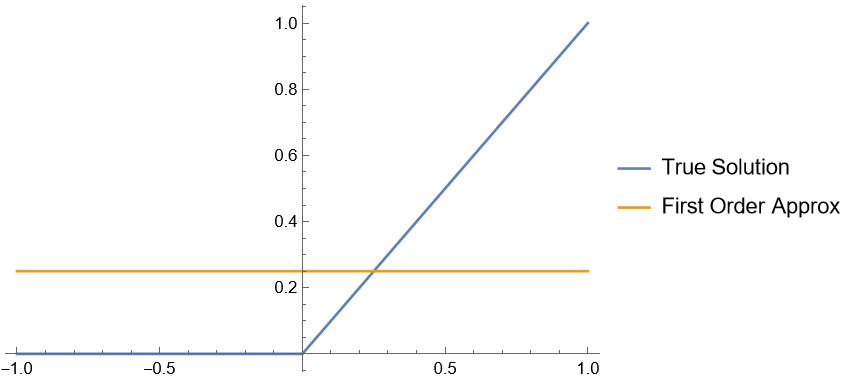
\includegraphics[width=\linewidth]{images/3-1.png}
            \caption{Approximation with one term.}
            \label{fig1:a}
            \vspace{4ex}
        \end{subfigure}%%
        \begin{subfigure}[b]{0.5\linewidth}
            \centering
            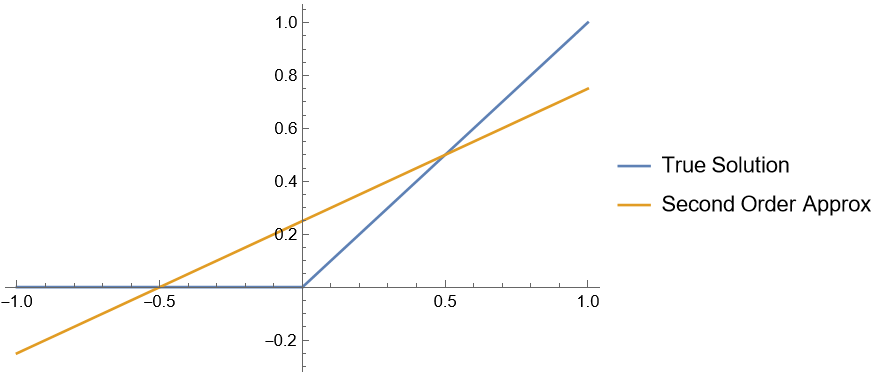
\includegraphics[width=\linewidth]{images/3-2.png}
            \caption{Approximation with two terms.}
            \label{fig1:b}
            \vspace{4ex}
        \end{subfigure}
        \begin{subfigure}[b]{0.5\linewidth}
            \centering
            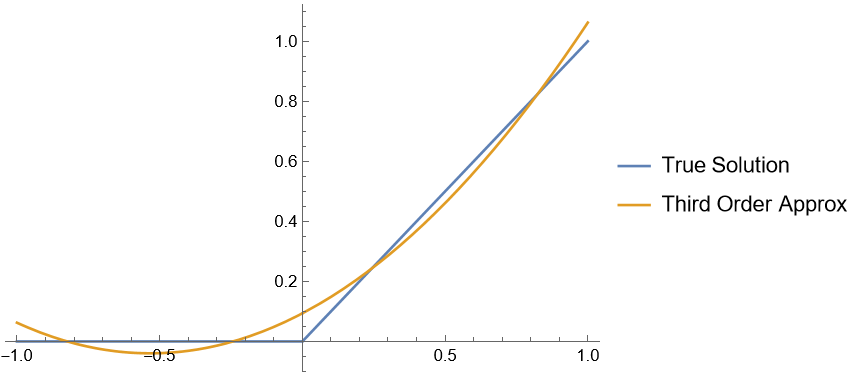
\includegraphics[width=\linewidth]{images/3-3.png}
            \caption{Approximation with three terms.}
            \label{fig1:c}
            \vspace{4ex}
        \end{subfigure}%%
        \begin{subfigure}[b]{0.5\linewidth}
            \centering
            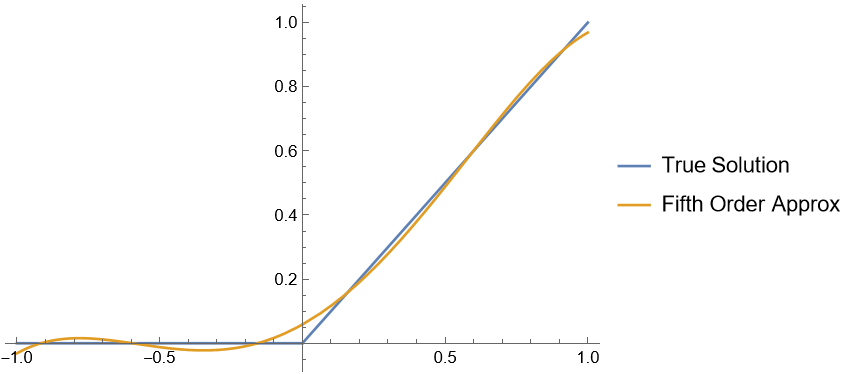
\includegraphics[width=\linewidth]{images/3-4.png}
            \caption{Approximation with four terms.}
            \label{fig1:d}
            \vspace{4ex}
        \end{subfigure}
        \caption{True solution to Legendre's equation seen in blue while different order Legendre expansion approximations in orange. }
        \label{fig1}
    \end{figure}



\end{solution}

%----------------------------------------------------------------------------------------------------%
%\vskip 20pt
\newpage


\end{document}